\documentclass{article}
\usepackage[english]{otex}
\addbibresource{ref.bib}

\ctexset{
    % otex宏包的[english]选项已自动处理了以下名称的英文本地化 (如 Contents, References 等)
    % 仅保留自定义的格式设置:
    section/format += \raggedright % (可选) 让章节标题左对齐而不是居中
}

% 文档元数据
\title{Orion's LaTeX Encyclopedia \\ \large \zh{LaTeX 权威指南与百科全书}}
\author{Orion \thanks{Email: orion@example.com}}
\date{\today}

\begin{document}

\maketitle

\begin{abstract}
    \noindent \textbf{Abstract:} This document serves as a comprehensive encyclopedia for LaTeX usage, designed to demonstrate the full capabilities of the \texttt{otex} package. It adopts a bilingual format (Chinese and English) and a structured four-step demonstration process for each feature: Introduction, Code, Explanation, and Effect. Topics covered include lists, mathematics, code algorithms, tables, figures, references, TikZ graphics, and advanced PGFPlots.
    
    \vspace{0.5em}
    \noindent \textbf{\zh{摘要:}} 本文档是一部全面的 LaTeX 使用百科全书,旨在展示 \texttt{otex} 宏包的强大功能。文档采用中英文双语格式,并对每个功能通过标准化的四步流程进行演示:功能介绍、代码展示、语法详解和效果展示。涵盖的主题包括列表、数学公式、算法代码、表格、插图、引用系统、TikZ 绘图以及高级 PGFPlots 数据可视化。
\end{abstract}

\tableofcontents
\newpage

% ==========================================================
\section{Lists and Enumerations (列表与枚举)}
% ==========================================================

\subsection{Unordered Lists (无序列表)}

\subsubsection{功能介绍 (Introduction)} 

无序列表用于展示没有特定顺序的项目集合。默认使用圆点作为符号,但可以通过 \texttt{enumitem} 宏包进行高度定制。

Unordered lists are used to display a collection of items with no specific order. They use bullets by default but can be highly customized using the \texttt{enumitem} package.

\vspace{0.5em}
\subsubsection{代码展示 (Code)}

\begin{minted}{latex}
\begin{itemize}
    \item Default item
    \item[--] Custom dash item
    \item[\textcolor{red}{$\bullet$}] Red bullet item
\end{itemize}
\end{minted}

\subsubsection{语法详解 (Syntax)}

\begin{itemize}
    \item \code{\textbackslash begin\{itemize\}}: 开启无序列表环境。
    \item \code{\textbackslash item}: 开始一个新列表项。
    \item \code{[label]}: 可选参数,用于覆盖默认符号 (需 \texttt{enumitem})。
    \item \code{\textbackslash bullet}: 默认的圆点符号。
\end{itemize}

\subsubsection{效果展示 (Effect)}

\begin{itemize}
    \item Default item
    \item[--] Custom dash item
    \item[\textcolor{red}{$\bullet$}] Red bullet item
\end{itemize}

% ----------------------------------------------------------

\subsection{Ordered Lists (有序列表)}

\subsubsection{功能介绍 (Introduction)} 

有序列表用于展示有顺序的步骤或排行。可以自动生成数字、字母或罗马数字编号。

Ordered lists are used to display sequential steps or rankings. They can automatically generate numbers, letters, or Roman numerals.

\vspace{0.5em}
\subsubsection{代码展示 (Code)}

\begin{minted}{latex}
\begin{enumerate}[label=\textbf{Step \arabic*.}]
    \item First step
    \item Second step
    \begin{enumerate}[label=(\alph*)]
        \item Sub-step A
        \item Sub-step B
    \end{enumerate}
\end{enumerate}
\end{minted}

\subsubsection{语法详解 (Syntax)}

\begin{itemize}
    \item \code{\textbackslash begin\{enumerate\}}: 开启有序列表环境。
    \item \code{label=\textbackslash arabic*}: 设置标签样式,\code{\textbackslash arabic*} 代表阿拉伯数字 (1, 2, 3)。
    \item \code{\textbackslash alph*}: 小写字母 (a, b, c)。
    \item \code{\textbackslash Roman*}: 大写罗马数字 (I, II, III)。
    \item \code{Step}: 可以在编号前后添加自定义文本。
\end{itemize}

\subsubsection{效果展示 (Effect)}

\begin{enumerate}[label=\textbf{Step \arabic*.}]
    \item First step
    \item Second step
    \begin{enumerate}[label=(\alph*)]
        \item Sub-step A
        \item Sub-step B
    \end{enumerate}
\end{enumerate}

% ----------------------------------------------------------

\subsection{Description Lists (描述列表)}

\subsubsection{功能介绍 (Introduction)} 

描述列表用于解释术语或定义概念,每个项目由一个加粗的标签和一段描述文本组成。

Description lists are used to explain terms or define concepts, where each item consists of a bold label and a description text.

\vspace{0.5em}
\subsubsection{代码展示 (Code)}

\begin{minted}{latex}
\begin{description}
    \item[LaTeX] A document preparation system.
    \item[CLI] Command Line Interface.
\end{description}
\end{minted}

\subsubsection{语法详解 (Syntax)}

\begin{itemize}
    \item \code{\textbackslash item[Label]}: 方括号内的内容会作为标签加粗显示。
\end{itemize}

\subsubsection{效果展示 (Effect)}

\begin{description}
    \item[LaTeX] A document preparation system used for high-quality typesetting.
    \item[CLI] Command Line Interface, interaction with computer programs via text.
\end{description}

% ----------------------------------------------------------

\subsection{Nested Lists (嵌套列表)}

\subsubsection{功能介绍 (Introduction)}

嵌套列表允许在列表项中创建子列表。LaTeX 自动为不同层级的列表处理标签样式(如:1 $\to$ (a) $\to$ i $\to$ A)。

Nested lists allow creating sub-lists within list items. LaTeX automatically handles label styles for different levels (e.g., 1 $\to$ (a) $\to$ i $\to$ A).

\vspace{0.5em}
\subsubsection{代码展示 (Code)}

\begin{minted}{latex}
\begin{enumerate}
    \item First top-level item
    \begin{enumerate}
        \item First sub-item
        \item Second sub-item
        \begin{enumerate}
            \item Deeply nested item
        \end{enumerate}
    \end{enumerate}
    \item Second top-level item
\end{enumerate}
\end{minted}

\subsubsection{语法详解 (Syntax)}

\begin{itemize}
    \item 嵌套列表最大深度默认为 4 层。
    \item \code{enumerate} 默认标签顺序:1, (a), i, A。
    \item \code{itemize} 默认标签顺序:$\bullet$, --, $\ast$, $\cdot$。
\end{itemize}

\subsubsection{效果展示 (Effect)}

\begin{enumerate}
    \item First top-level item
    \begin{enumerate}
        \item First sub-item
        \item Second sub-item
        \begin{enumerate}
            \item Deeply nested item
        \end{enumerate}
    \end{enumerate}
    \item Second top-level item
\end{enumerate}

% ----------------------------------------------------------

\subsection{Custom List Styles (自定义列表样式)}

\subsubsection{功能介绍 (Introduction)}

利用 \texttt{enumitem} 宏包,可以轻松修改列表的符号、编号样式、间距等。

Using the \texttt{enumitem} package, you can easily modify list symbols, numbering styles, spacing, etc.

\vspace{0.5em}
\subsubsection{代码展示 (Code)}

\begin{minted}{latex}
% Resume numbering from previous list
\begin{enumerate}[resume]
    \item Third item (continued)
\end{enumerate}

% Custom symbol and color
\begin{itemize}[label=\textcolor{blue}{\textbullet}]
    \item Blue bullet item
\end{itemize}

% Roman numerals with custom format
\begin{enumerate}[label=\Roman*., start=5]
    \item Item V
    \item Item VI
\end{enumerate}
\end{minted}

\subsubsection{语法详解 (Syntax)}

\begin{itemize}
    \item \code{resume}: 接续上前一个同类型列表的编号。
    \item \code{start=N}: 强制从数字 N 开始编号。
    \item \code{label=\textbackslash textcolor\{color\}\{symbol\}}: 自定义标签颜色和符号。
\end{itemize}

\subsubsection{效果展示 (Effect)}

\begin{enumerate}
    \item Previous item 1
    \item Previous item 2
\end{enumerate}

\begin{enumerate}[resume]
    \item Third item (continued numbering)
\end{enumerate}

\begin{itemize}[label=\textcolor{blue}{\textbullet}]
    \item Blue bullet item
\end{itemize}

\begin{enumerate}[label=\Roman*., start=5]
    \item Item V
    \item Item VI
\end{enumerate}

% ----------------------------------------------------------

\subsection{Inline Lists (行内列表)}

\subsubsection{功能介绍 (Introduction)}

行内列表用于在段落文字中穿插列表项,通常用于枚举短语。需要 \texttt{enumitem} 的 \texttt{inline} 选项(本模板已默认加载)。

Inline lists are used to intersperse list items within paragraph text, typically for enumerating phrases. Requires the \texttt{inline} option of \texttt{enumitem} (loaded by default in this template).

\vspace{0.5em}
\subsubsection{代码展示 (Code)}

\begin{minted}{latex}
Three things to remember:
\begin{enumerate*}[label=(\arabic*)]
    \item practice,
    \item practice, and
    \item more practice.
\end{enumerate*}
\end{minted}

\subsubsection{语法详解 (Syntax)}

\begin{itemize}
    \item \code{enumerate*}: 行内有序列表环境 (需 \texttt{enumitem[inline]})。
    \item \code{itemize*}: 行内无序列表环境。
    \item 适用于将列表项作为句子的一部分流畅展示。
\end{itemize}

\subsubsection{效果展示 (Effect)}

Three things to remember:
\begin{enumerate*}[label=(\arabic*)]
    \item practice,
    \item practice, and
    \item more practice.
\end{enumerate*}

% ----------------------------------------------------------

\subsection{Checklists (任务清单)}

\subsubsection{功能介绍 (Introduction)}

使用 \texttt{amssymb} 提供的符号创建待办事项清单。

Create to-do lists using symbols provided by \texttt{amssymb}.

\vspace{0.5em}
\subsubsection{代码展示 (Code)}

\begin{minted}{latex}
\begin{itemize}[label=$\square$]
    \item Unchecked task
    \item[$\boxtimes$] Checked task
    \item Another pending task
\end{itemize}
\end{minted}

\subsubsection{语法详解 (Syntax)}

\begin{itemize}
    \item \code{\textbackslash square}: 空方框符号 (需 \texttt{amssymb})。
    \item \code{\textbackslash boxtimes}: 带叉方框符号。
    \item \code{\textbackslash checkmark}: 对勾符号。
\end{itemize}

\subsubsection{效果展示 (Effect)}

\begin{itemize}[label=$\square$]
    \item Unchecked task
    \item[$\boxtimes$] Checked task
    \item Another pending task
\end{itemize}


\newpage
% ==========================================================
\section{Mathematics (数学公式)}
% ==========================================================

\subsection{Equations and Alignments (方程与对齐)}

\subsubsection{功能介绍 (Introduction)} 

LaTeX 最强大的功能之一是排版数学公式。我们可以使用 \texttt{equation} 环境进行自动编号,使用 \texttt{align} 环境进行多行公式对齐。

One of LaTeX's most powerful features is typesetting mathematics. We can use the \texttt{equation} environment for automatic numbering and the \texttt{align} environment for multi-line equation alignment.

\vspace{0.5em}
\subsubsection{代码展示 (Code)}

\begin{minted}{latex}
% Single numbered equation
\begin{equation}
    E = mc^2 \label{eq:einstein}
\end{equation}

% Aligned equations
\begin{align}
    f(x) &= (x+a)(x+b) \nonumber \\
         &= x^2 + (a+b)x + ab
\end{align}
\end{minted}

\subsubsection{语法详解 (Syntax)}

\begin{itemize}
    \item \code{equation}: 生成带编号的单行公式。
    \item \code{align}: 生成多行公式,使用 \code{\&} 指定对齐位置,反斜杠加反斜杠换行。
    \item \code{nonumber}: 阻止当前行生成编号。
    \item \code{label}: 添加引用标签。
\end{itemize}

\subsubsection{效果展示 (Effect)}

\begin{equation}
    E = mc^2 \label{eq:einstein}
\end{equation}

\begin{align}
    f(x) &= (x+a)(x+b) \nonumber \\
         &= x^2 + (a+b)x + ab
\end{align}

% ----------------------------------------------------------

\subsection{Matrices and Cases (矩阵与分段函数)}

\subsubsection{功能介绍 (Introduction)} 

矩阵和分段函数是线性代数和微积分中常见的结构。

Matrices and piecewise functions are common structures in linear algebra and calculus.

\vspace{0.5em}
\subsubsection{代码展示 (Code)}

\begin{minted}{latex}
$$
    \mathbf{A} = \begin{pmatrix} 
        1 & 0 \\ 
        0 & 1 
    \end{pmatrix}, 
    \quad
    |x| = \begin{cases}
        x & \text{if } x \ge 0 \\
        -x & \text{if } x < 0
    \end{cases}
$$
\end{minted}

\subsubsection{语法详解 (Syntax)}

\begin{itemize}
    \item \code{pmatrix}: 圆括号矩阵 \code{()}。
    \item \code{bmatrix}: 方括号矩阵 \code{[]}。
    \item \code{cases}: 分段函数环境,自动添加左大括号。
    \item \code{\textbackslash text}: 在数学模式中插入普通文本。
\end{itemize}

\subsubsection{效果展示 (Effect)}

$$
    \mathbf{A} = \begin{pmatrix} 
        1 & 0 \\ 
        0 & 1 
    \end{pmatrix}, 
    \quad
    |x| = \begin{cases}
        x & \text{if } x \ge 0 \\
        -x & \text{if } x < 0
    \end{cases}
$$

% ----------------------------------------------------------

\subsection{Calculus and Integrals (微积分与积分)}

\subsubsection{功能介绍 (Introduction)}

微积分公式通常包含极限、求和、积分等复杂的上下标结构。使用 \texttt{\$\$} 可以让这些公式独立成行显示。

Calculus formulas often involve complex limits, sums, and integrals with subscripts and superscripts. Using \texttt{\$\$} displays these formulas on their own lines.

\vspace{0.5em}
\subsubsection{代码展示 (Code)}

\begin{minted}{latex}
% Limit and Summation
$$ \lim_{x \to \infty} \frac{1}{x} = 0, \quad \sum_{n=1}^{\infty} \frac{1}{n^2} = \frac{\pi^2}{6} $$

% Definite Integral
$$ \int_{a}^{b} f(x) \,dx = F(b) - F(a) $$

% Triple Integral
$$ \iiint_{V} \rho(x,y,z) \,dx\,dy\,dz $$
\end{minted}

\subsubsection{语法详解 (Syntax)}

\begin{itemize}
    \item \code{\textbackslash lim}, \code{\textbackslash sum}, \code{\textbackslash int}: 分别表示极限、求和、积分。
    \item \code{\_\{...\}}: 下标 (Lower limit)。
    \item \code{\^\{...\}}: 上标 (Upper limit)。
    \item \code{\textbackslash to}: 趋近箭头 ($\to$)。
    \item \code{\textbackslash infty}: 无穷符号 ($\infty$)。
    \item \code{\textbackslash,}: 插入一个小间距 (thin space),常用于微分算子 $dx$ 前。
\end{itemize}

\subsubsection{效果展示 (Effect)}

$$ \lim_{x \to \infty} \frac{1}{x} = 0, \quad \sum_{n=1}^{\infty} \frac{1}{n^2} = \frac{\pi^2}{6} $$

$$ \int_{a}^{b} f(x) \,dx = F(b) - F(a) $$

$$ \iiint_{V} \rho(x,y,z) \,dx\,dy\,dz $$

% ----------------------------------------------------------

\subsection{Theorem Environments (定理环境)}

\subsubsection{功能介绍 (Introduction)}

\texttt{otex.sty} 预定义了常用的数学环境,如定理、定义、引理和证明。这些环境会自动处理编号和格式。

\texttt{otex.sty} predefines common mathematical environments such as theorems, definitions, lemmas, and proofs. These environments automatically handle numbering and formatting.

\vspace{0.5em}
\subsubsection{代码展示 (Code)}

\begin{minted}{latex}
\begin{definition}[Prime Number]
    A natural number greater than 1 that has no positive divisors other than 1 and itself.
\end{definition}

\begin{theorem}[Euclid]
    There are infinitely many prime numbers.
\end{theorem}

\begin{proof}
    Suppose there are finitely many primes $p_1, \dots, p_n$. Let $P = p_1 \cdots p_n + 1$. Then $P$ is not divisible by any $p_i$, contradiction.
\end{proof}
\end{minted}

\subsubsection{语法详解 (Syntax)}

\begin{itemize}
    \item \code{definition}: 定义环境。
    \item \code{theorem}: 定理环境,可选参数 \code{[Name]} 用于指定定理名称。
    \item \code{proof}: 证明环境,自动以 Q.E.D. 方块结尾。
    \item 更多可用环境: \code{lemma} (引理), \code{proposition} (命题), \code{corollary} (推论), \code{example} (例), \code{remark} (注).
\end{itemize}

\paragraph{配置定理名称 (Configuring Names)}

可以通过加载宏包时的选项或重定义宏来修改环境名称。

You can change the environment names by passing package options or redefining macros.

\begin{minted}{latex}
% Option 1: Use English names (Theorem, Definition, etc.)
% \usepackage[english]{otex}

% Option 2: Manually redefine specific names
\renewcommand{\algorithmcfname}{算法} % Rename algorithm
\renewcommand{\theoremname}{MyTheorem} % Custom theorem name
\end{minted}

\subsubsection{效果展示 (Effect)}

\begin{definition}[Prime Number]
    A natural number greater than 1 that has no positive divisors other than 1 and itself.
\end{definition}

\begin{theorem}[Euclid]
    There are infinitely many prime numbers.
\end{theorem}

\begin{proof}
    Suppose there are finitely many primes $p_1, \dots, p_n$. Let $P = p_1 \cdots p_n + 1$. Then $P$ is not divisible by any $p_i$, contradiction.
\end{proof}

% ----------------------------------------------------------

\subsection{Greek Letters and Special Symbols (希腊字母与特殊符号)}

\subsubsection{功能介绍 (Introduction)}

LaTeX 提供了大量的数学符号。以下是一些常用的希腊字母和关系符号的示例。

LaTeX provides a vast array of mathematical symbols. Below are examples of common Greek letters and relation symbols.

\vspace{0.5em}
\subsubsection{代码展示 (Code)}

\begin{minted}{latex}
$$
    \alpha, \beta, \gamma, \Delta, \pi, \theta, \phi
$$
$$
    \forall x \in \mathbb{R}, \exists y \text{ s.t. } y > x
$$
$$
    A \subseteq B, \quad A \cup B, \quad A \cap B, \quad x \neq y
$$
\end{minted}

\subsubsection{语法详解 (Syntax)}

\begin{itemize}
    \item 希腊字母: \code{\textbackslash alpha}, \code{\textbackslash beta}, \code{\textbackslash Delta} (大写), 等。
    \item 逻辑符号: \code{\textbackslash forall} ($\forall$), \code{\textbackslash exists} ($\exists$)。
    \item 集合符号: \code{\textbackslash in} ($\in$), \code{\textbackslash subseteq} ($\subseteq$), \code{\textbackslash cup} ($\cup$), \code{\textbackslash cap} ($\cap$)。
    \item \code{\textbackslash mathbb}: 黑板粗体,常用于表示数集 (需 \code{amssymb} 宏包)。
\end{itemize}

\subsubsection{效果展示 (Effect)}

$$
    \alpha, \beta, \gamma, \Delta, \pi, \theta, \phi
$$
$$
    \forall x \in \mathbb{R}, \exists y \text{ s.t. } y > x
$$
$$
    A \subseteq B, \quad A \cup B, \quad A \cap B, \quad x \neq y
$$

% ==========================================================


\newpage
% ==========================================================
\section{Code and Algorithms (代码与算法)}
% ==========================================================

\subsection{Code Listings (代码块)}

\subsubsection{功能介绍 (Introduction)} 

展示源代码时,通常需要语法高亮、行号和等宽字体。我们推荐使用 \texttt{minted} 宏包 (基于 Pygments) 来实现更优质的高亮效果。

When displaying source code, syntax highlighting, line numbers, and monospaced fonts are usually required. We recommend using the \texttt{minted} package (based on Pygments) for superior highlighting.

\vspace{0.5em}
\subsubsection{代码展示 (Code)}

\begin{lstlisting}[language=TeX]
\begin{listing}[H]
    \caption{Python Example}
    \label{lst:py}
    \begin{minted}{python}
def factorial(n):
    if n == 0:
        return 1
    return n * factorial(n-1)
    \end{minted}
\end{listing }
\end{lstlisting}

\subsubsection{语法详解 (Syntax)}

\begin{itemize}
    \item \code{minted}: 环境名称。
    \item \code{\{python\}}: 必选参数,指定语言。
    \item \code{listing}: 可选的浮动环境,用于承载 \code{caption} 和 \code{label}。
\end{itemize}

\subsubsection{效果展示 (Effect)}

\begin{listing}[H]
    \caption{Python Recursive Factorial}
    \label{lst:py}
    \begin{minted}{python}
def factorial(n):
    """Calculate the factorial of n recursively."""
    if n == 0:
        return 1
    else:
        return n * factorial(n-1)
    \end{minted}
\end{listing}

% ----------------------------------------------------------

\subsection{Algorithms (伪代码)}

\subsubsection{功能介绍 (Introduction)} 

算法伪代码提供了一种结构化的方式来描述算法逻辑,独立于具体编程语言。

Algorithm pseudocode provides a structured way to describe algorithmic logic, independent of specific programming languages.

\vspace{0.5em}
\subsubsection{代码展示 (Code)}

\begin{minted}{latex}
\begin{algorithm}[H]
    \SetAlgoLined
    \KwIn{List $L$}
    \KwOut{Sorted List $L$}
    \While{unsorted}{
        Find minimum element $m$\;
        Move $m$ to sorted portion\;
    }
    \caption{Selection Sort}
\end{algorithm}
\end{minted}

\subsubsection{语法详解 (Syntax)}

\begin{itemize}
    \item \code{algorithm2e}: 使用的宏包。
    \item \code{\KwIn}, \code{\KwOut}: 输入输出关键字。
    \item \code{\While}, \code{\If}: 控制流结构。
    \item \code{\textbackslash;}: 语句结束的分号。
\end{itemize}

\subsubsection{效果展示 (Effect)}

\begin{algorithm}[H]
    \SetAlgoLined
    \KwIn{Array $A$ of $n$ elements}
    \KwOut{Sorted Array $A$}
    \For{$i \gets 0$ \KwTo $n-2$}{
        $\min \gets i$\;
        \For{$j \gets i+1$ \KwTo $n-1$}{
            \If{$A[j] < A[\min]$}{
                $\min \gets j$\;
            }
        }
        Swap $A[i]$ and $A[\min]$\;
    }
    \caption{Selection Sort Algorithm}
\end{algorithm}


\newpage
% ==========================================================
\section{Tables (表格)}
% ==========================================================

\subsection{Professional Tables (专业表格)}

\subsubsection{功能介绍 (Introduction)} 

科技论文中推荐使用所有的 ``三线表'',即仅使用顶部、中部和底部三条横线,去除垂直分割线。

Scientific papers recommend using "Three-line Tables", which use only top, middle, and bottom horizontal lines, removing vertical separators.

\vspace{0.5em}
\subsubsection{代码展示 (Code)}

\begin{minted}{latex}
\begin{table}[htbp]
    \centering
    \caption{Comparison of Metrics}
    \begin{tabular}{l c r}
        \toprule
        \textbf{Model} & \textbf{Accuracy} & \textbf{Time (s)} \\
        \midrule
        Baseline & 85.2\% & 12.5 \\
        Ours & 92.1\% & 15.3 \\
        \bottomrule
    \end{tabular}
\end{table}
\end{minted}

\subsubsection{语法详解 (Syntax)}

\textbf{Tabular 环境基础}:
\begin{minted}{latex}
\begin{tabular}{col_spec}
    Cell 1 & Cell 2 \\ 
    ...
\end{tabular}
\end{minted}

\begin{itemize}
    \item \textbf{列格式 (Column Specifiers)}: 定义在 \code{\begin{tabular}} 后的花括号中。
    \begin{itemize}
        \item \code{l}: 左对齐 (Left-aligned column)。
        \item \code{c}: 居中对齐 (Centered column)。
        \item \code{r}: 右对齐 (Right-aligned column)。
        \item \code{p{width}}: 指定宽度的段落列,内容会自动换行 (Paragraph column with fixed width, supports auto-wrapping)。
        \item \code{|}: 绘制垂直分割线 (Vertical line)。例如 \code{|c|c|} 表示两列都有边框。
    \end{itemize}
    \item \textbf{行与列分隔}:
    \begin{itemize}
        \item \code{\&}: 分隔同一行中的不同列 (Separates columns).
        \item \code{\\}: 结束当前行 (Ends the current row).
    \end{itemize}
    \item \code{booktabs}: 提供 \code{\toprule}, \code{\midrule}, \code{\bottomrule} 以绘制不同粗细的专业横线,替代标准的 \code{\hline}。
\end{itemize}

\subsubsection{效果展示 (Effect)}

\begin{table}[htbp]
    \centering
    \caption{Comparison of Accuracy and Performance}
    \begin{tabular}{l c r}
        \toprule
        \textbf{Model} & \textbf{Accuracy} & \textbf{Inference Time (ms)} \\
        \midrule
        ResNet-50 & 76.1\% & 24 \\
        ViT-Base & 81.3\% & 45 \\
        \textbf{Ours-Pro} & \textbf{83.5\%} & 38 \\
        \bottomrule
    \end{tabular}
\end{table}

\subsection{Column and Row Merging Fundamentals (行列合并基础)}

表格的高级功能核心在于“合并”。理解合并的关键在于:\textbf{表格本质上是一个网格,合并操作只是让某个单元格占据了邻近单元格的空间,但并未改变网格的底层逻辑。}

The core of advanced tables lies in "merging". The key is to understand that a table is a grid; merging simply allows a cell to occupy the space of its neighbors without changing the underlying grid logic.

\subsubsection{合并列 (\\multicolumn)}

合并列通过 \code{\multicolumn} 命令实现。它不仅用于合并,也常用于改变单个单元格的对齐方式(例如表头居中,数据居左)。

Column merging is done via \code{\multicolumn}. It is also used to change the alignment of a single cell.

\textbf{语法 (Syntax):}
\begin{minted}{latex}
\multicolumn{number}{align}{text}
\end{minted}
\begin{itemize}
    \item \code{number}: 要合并的列数 (Number of columns to merge)。
    \item \code{align}: 新的对齐方式 (e.g., \code{c}, \code{l}, \code{r}, \code{|c|})。
    \item \code{text}: 单元格内容。
\end{itemize}

\textbf{示例分析 (Example Analysis):}
我们想把第一行的两个单元格合并。

\begin{minted}{latex}
\begin{tabular}{|c|c|}
    \hline
    % 合并2列,居中对齐,内容为 "Title"
    \multicolumn{2}{|c|}{Merged Header} \\ 
    \hline
    Cell A & Cell B \\
    \hline
\end{tabular}
\end{minted}

\begin{center}
\begin{tabular}{|c|c|}
    \hline
    \multicolumn{2}{|c|}{\textbf{Merged Header}} \\ 
    \hline
    Cell A & Cell B \\
    \hline
\end{tabular}
\end{center}

\subsubsection{合并行 (\\multirow)}

合并行需要 \code{multirow} 宏包,命令为 \code{\multirow}。

Row merging requires the \code{multirow} package.

\textbf{语法 (Syntax):}
\begin{minted}{latex}
\multirow{number}{width}{text}
\end{minted}
\begin{itemize}
    \item \code{number}: 要合并的行数。
    \item \code{width}: 单元格宽度,通常填 \code{*} 让其自动适应。
    \item \code{text}: 单元格内容。
\end{itemize}

\textbf{重要规则 (Crucial Rule):}
当使用了 \code{\multirow{2}{...}} 时,当前行占据了位置。\textbf{在下一行对应的位置必须留空}(即直接写 \code{\&} 而不填内容),否则内容会重叠。

When using \code{\\multirow}, the corresponding cell in the \textbf{next rows} must be left empty.

\textbf{示例分析 (Example Analysis):}

\begin{minted}{latex}
\begin{tabular}{|c|c|}
    \hline
    % 第1行:声明合并2行,内容 "Common"
    \multirow{2}{*}{Common} & Row 1 Data \\ \cline{2-2}
    % 第2行:第一列留空!因为被上面占用了
     & Row 2 Data \\ 
    \hline
\end{tabular}
\end{minted}

\begin{center}
\begin{tabular}{|c|c|}
    \hline
    \multirow{2}{*}{Common} & Row 1 Data \\ \cline{2-2}
     & Row 2 Data \\ 
    \hline
\end{tabular}
\end{center}

注意使用 \code{\cline{2-2}} 来只画第2列的横线,否则会穿过 "Common" 文本。

Notice using \code{\cline{2-2}} to draw a horizontal line only across the 2nd column.

\subsection{Step-by-Step Complex Table (手把手构建复杂表格)}

让我们构建一个复杂的“课程表”,包含多级表头。

Let's build a complex "Schedule" with multi-level headers.

\textbf{目标结构 (Goal Logic):}
\begin{itemize}
    \item 总共4列。
    \item 表头第1列是 "Day" (需要跨越3行: Header 1, 2, 3)。
    \item 表头第2-4列是 "Schedule" (跨越3列)。
    \item "Schedule" 下面分为 "Morning" (跨越1列, 跨越2行) 和 "Afternoon" (跨越2列)。
    \item "Afternoon" 下面分为 "13:00" 和 "15:00"。
\end{itemize}

\textbf{代码实现 (Implementation):}

\begin{minted}{latex}
\begin{table}[htbp]
\centering
\caption{Complex Schedule Construction}
\begin{tabular}{l c c c}
    \toprule
    % --- Row 1 ---
    % Col 1: Day (跨3行)
    % Col 2-4: Schedule (跨3列)
    \multirow{3}{*}{\textbf{Day}} & \multicolumn{3}{c}{\textbf{Schedule}} \\ 
    % 绘制横线: 从第2列到第4列 (不穿过Day)
    \cmidrule(lr){2-4}
    
    % --- Row 2 ---
    % Col 1: 空 (Day占位)
    % Col 2: Morning (跨2行)
    % Col 3-4: Afternoon (跨2列)
     & \multirow{2}{*}{\textbf{Morning}} & \multicolumn{2}{c}{\textbf{Afternoon}} \\ 
    % 绘制横线: 从第3列到第4列 (Morning下方不画线)
    \cmidrule(lr){3-4}
    
    % --- Row 3 ---
    % Col 1: 空 (Day占位)
    % Col 2: 空 (Morning占位)
    % Col 3: 13:00
    % Col 4: 15:00
     & & \textbf{13:00} & \textbf{15:00} \\ 
    \midrule
    
    % --- Data Rows ---
    Mon & Math & Physics & History \\
    Tue & CS & \multicolumn{2}{c}{Lab (3 hours)} \\ % 数据也可以合并
    \bottomrule
\end{tabular}
\end{table}
\end{minted}

\subsubsection{最终效果 (Final Effect)}

\begin{table}[htbp]
\centering
\caption{Complex Schedule Construction}
\begin{tabular}{l c c c}
    \toprule
    \multirow{3}{*}{\textbf{Day}} & \multicolumn{3}{c}{\textbf{Schedule}} \\ 
    \cmidrule(lr){2-4}
     & \multirow{2}{*}{\textbf{Morning}} & \multicolumn{2}{c}{\textbf{Afternoon}} \\ 
    \cmidrule(lr){3-4}
     & & \textbf{13:00} & \textbf{15:00} \\ 
    \midrule
    Mon & Math & Physics & History \\
    Tue & CS & \multicolumn{2}{c}{Lab (3 hours)} \\
    \bottomrule
\end{tabular}
\end{table}

\subsection{Colored Tables (彩色表格)}

\subsubsection{功能介绍 (Introduction)}
通过 \code{xcolor} 宏包的 \code{table} 选项,可以轻松为表格添加背景色。

\vspace{0.5em}
\subsubsection{代码展示 (Code)}
\begin{minted}{latex}
% \usepackage[table]{xcolor}
\begin{tabular}{l c}
    \toprule
    % 行颜色
    \rowcolor{blue!10} \textbf{Item} & \textbf{Cost} \\
    \midrule
    Apple & \$1.00 \\
    % 单元格颜色覆盖行颜色
    Banana & \cellcolor{red!10} \$0.80 \\
    \bottomrule
\end{tabular}
\end{minted}

\subsubsection{颜色格式详解 (Color Syntax)}
\code{xcolor} 提供了强大的颜色混合语法。

\begin{itemize}
    \item \textbf{基础颜色}: \code{red}, \code{blue}, \code{green}, \code{black}, \code{white}, \code{yellow}, \code{cyan}, \code{magenta}.
    \item \textbf{透明度/混合 (Mixing)}: 
    \begin{itemize}
        \item \code{blue!40}: 40\% 蓝色 + 60\% 白色 (40\% Blue, 60\% White).
        \item \code{red!30!black}: 30\% 红色 + 70\% 黑色 (30\% Red mixed with Black).
        \item \code{blue!50!green}: 50\% 蓝色 + 50\% 绿色 (Mix Blue and Green).
    \end{itemize}
    \item \textbf{自定义颜色 (Custom Colors)}:
    \begin{minted}{latex}
\definecolor{myblue}{RGB}{0, 100, 200}    % 0-255 RGB
\definecolor{myred}{HTML}{FF0000}         % Hex
\definecolor{mygray}{gray}{0.9}           % 0-1 Grayscale
    \end{minted}
\end{itemize}

\subsubsection{效果展示 (Effect)}
\begin{table}[htbp]
    \centering
    \caption{Colorful Table Example}
    \begin{tabular}{l c}
        \toprule
        \rowcolor{blue!10} \textbf{Item} & \textbf{Cost} \\
        \midrule
        Apple & \$1.00 \\
        Banana & \cellcolor{red!10} \$0.80 \\
        \bottomrule
    \end{tabular}
\end{table}

\subsection{Long Tables (跨页长表格)}

\subsubsection{功能介绍 (Introduction)}
对于超过一页的表格,使用 \code{longtable} 环境。

\begin{minted}{latex}
\begin{longtable}{l p{8cm}}
    \caption{Long Table} \\
    \toprule
    Header 1 & Header 2 \\
    \midrule
    \endfirsthead
    % ... (后续页表头定义) ...
    \endhead
    % ... (页脚定义) ...
    \endfoot
    % ... (最后页脚定义) ...
    \endlastfoot
    
    Row 1 & Data... \\
    Row 2 & Data... \\
\end{longtable}
\end{minted}

\subsubsection{效果展示 (Effect)}
\begin{longtable}{l p{8cm}}
    \caption{Long Table Example} \\
    \toprule
    \textbf{Header 1} & \textbf{Header 2} \\
    \midrule
    \endfirsthead
    \multicolumn{2}{c}%
    {{\bfseries \tablename\ \thetable{} -- continued}} \\
    \toprule
    \textbf{Header 1} & \textbf{Header 2} \\
    \midrule
    \endhead
    \midrule
    \multicolumn{2}{r}{{Continued...}} \\
    \bottomrule
    \endfoot
    \bottomrule
    \endlastfoot
    
    Row 1 & Data for row 1 which might be long. \\
    Row 2 & Data for row 2 which might be long. \\
    Row 3 & Data for row 3 which might be long. \\
    Row 4 & Data for row 4 which might be long. \\
    Row 5 & Data for row 5 which might be long. \\
    Row 6 & Data for row 6 which might be long. \\
\end{longtable}


\newpage
% ==========================================================
\section{Figures (图片)}
% ==========================================================

\subsection{Standard Figures (标准插图)}

\subsubsection{功能介绍 (Introduction)} 

插入图片是文档排版的基本需求。LaTeX 使用 \texttt{figure} 浮动体环境来管理图片位置。

Inserting images is a basic requirement for document typesetting. LaTeX uses the \texttt{figure} floating environment to manage image placement.

\vspace{0.5em}
\subsubsection{代码展示 (Code)}

\begin{minted}{latex}
\begin{figure}[htbp]
    \centering
    \includegraphics[width=0.4\textwidth]{example-image-a}
    \caption{Standard Figure}
    \label{fig:std}
\end{figure}
\end{minted}

\subsubsection{语法详解 (Syntax)}

\begin{itemize}
    \item \code{\textbackslash includegraphics[options]\{file\}}: 插入图片。
    \item \code{width=0.4\textbackslash textwidth}: 设置宽度为文本宽度的 40\%。
    \item \code{[htbp]}: 推荐的位置参数 (Here, Top, Bottom, Page)。
\end{itemize}

\subsubsection{效果展示 (Effect)}

\begin{figure}[htbp]
    \centering
    \includegraphics[width=0.4\textwidth]{example-image-a}
    \caption{Standard Figure Example}
    \label{fig:std-example}
\end{figure}

% ----------------------------------------------------------

\subsection{Subfigures (子图)}

\subsubsection{功能介绍 (Introduction)} 

当需要对比多张图片时,可以使用子图功能。

When comparing multiple images, subfigures are useful.

\vspace{0.5em}
\subsubsection{代码展示 (Code)}

\begin{minted}{latex}
\begin{figure}[htbp]
    \centering
    \begin{subfigure}[b]{0.3\textwidth}
        \includegraphics[width=\textwidth]{example-image-b}
        \caption{Left}
    \end{subfigure}
    \hfill
    \begin{subfigure}[b]{0.3\textwidth}
        \includegraphics[width=\textwidth]{example-image-c}
        \caption{Right}
    \end{subfigure}
    \caption{Comparison}
\end{figure}
\end{minted}

\subsubsection{语法详解 (Syntax)}

\begin{itemize}
    \item \code{subcaption}: 宏包提供的 \code{subfigure} 环境。
    \item \code{\textbackslash hfill}: 在两个子图之间插入弹性空格以撑满行宽。
\end{itemize}

\subsubsection{效果展示 (Effect)}

\begin{figure}[htbp]
    \centering
    \begin{subfigure}[b]{0.3\textwidth}
        \includegraphics[width=\textwidth]{example-image-b}
        \caption{Method A}
    \end{subfigure}
    \hfill
    \begin{subfigure}[b]{0.3\textwidth}
        \includegraphics[width=\textwidth]{example-image-c}
        \caption{Method B}
    \end{subfigure}
    \caption{Subfigure Comparison Example}
\end{figure}

% ----------------------------------------------------------

\subsection{Text Wrapping (图文环绕)}

\subsubsection{功能介绍 (Introduction)} 

当需要文字环绕图片排列时(常见于杂志或教材排版),可以使用 \texttt{wrapfigure} 环境。请注意,不需要环绕的文字段落长度必须足够包围图片。

When text needs to wrap around an image (common in magazine or textbook layouts), use the \texttt{wrapfigure} environment. Note that the text paragraph must be long enough to wrap around the image.

\vspace{0.5em}
\subsubsection{代码展示 (Code)}

\begin{minted}{latex}
\begin{wrapfigure}{r}{0.3\textwidth}
    \centering
    \includegraphics[width=0.25\textwidth]{example-image}
    \caption{Wrapped Image}
\end{wrapfigure}
This text wraps around the figure on the right. 
Make sure there is enough text content here...
\end{minted}

\subsubsection{语法详解 (Syntax)}

\begin{itemize}
    \item \code{\textbackslash begin\{wrapfigure\}\{align\}\{width\}}: 开启环绕环境。
    \item \code{align}: 对齐方式,\code{r} (right), \code{l} (left)。大写 \code{R}/\code{L} 表示浮动。
    \item \code{width}: 图片占用的总宽度。
\end{itemize}

\subsubsection{效果展示 (Effect)}

\begin{wrapfigure}{r}{0.3\textwidth}
    \centering
    \includegraphics[width=0.25\textwidth]{example-image}
    \caption{Wrapped Image}
\end{wrapfigure}
Lorem ipsum dolor sit amet, consectetuer adipiscing elit. Etiam lobortis facilisis sem. Nullam nec mi et neque pharetra sollicitudin. Praesent imperdiet mi nec ante. Donec ullamcorper, felis non sodales commodo, lectus velit ultrices augue, a dignissim nibh lectus placerat pede. Vivamus nunc nunc, molestie ut, ultricies vel, semper in, velit. Ut porta, leo ut ultricies aliquam, odio wisi commodo quam, vel accumsan dolor wisi et ante. Pellentesque habitant morbi tristique senectus et netus et malesuada fames ac turpis egestas.
\par % Ensure paragraph ends to clear wrapping correctly if needed


\newpage
% ==========================================================
\section{References and Alerts (引用与提示)}
% ==========================================================

\subsection{Citations and Cross-References (引用)}

\subsubsection{功能介绍 (Introduction)} 

自动化管理参考文献和交叉引用是 LaTeX 的核心优势。

Automated management of bibliography and cross-references is a core strength of LaTeX.

\vspace{0.5em}
\subsubsection{代码展示 (Code)}

\begin{minted}{latex}
See Figure \ref{fig:std} on page \pageref{fig:std}.
As shown in \cite{shannon1948}, information theory...
\end{minted}

\subsubsection{语法详解 (Syntax)}

\begin{itemize}
    \item \code{\ref{key}}: 引用编号。
    \item \code{\pageref{key}}: 引用页码。
    \item \code{\cite{key}}: 引用参考文献。
\end{itemize}

\subsubsection{效果展示 (Effect)} 

See Figure \ref{fig:std-example} on page \pageref{fig:std-example}. \\

As shown in \cite{shannon1948}, information theory is fundamental to modern communication.

% ----------------------------------------------------------

\subsection{Alert Boxes (提示框)}

\subsubsection{功能介绍 (Introduction)} 

使用 \texttt{tcolorbox} 创建醒目的提示框。

Use \texttt{tcolorbox} to create eye-catching alert boxes.

\vspace{0.5em}
\subsubsection{代码展示 (Code)}

\begin{minted}{latex}
\begin{tcolorbox}[colback=red!5!white,colframe=red!75!black,title=Warning]
    This is a warning!
\end{tcolorbox}
\end{minted}

\subsubsection{语法详解 (Syntax)}

\begin{itemize}
    \item \code{colback}: 背景色。
    \item \code{colframe}: 边框色。
    \item \code{title}: 盒子标题。
\end{itemize}

\subsubsection{效果展示 (Effect)}

\begin{tcolorbox}[colback=red!5!white,colframe=red!75!black,title=Warning]
    Please pay attention to this critical warning.
\end{tcolorbox}


\newpage
% ==========================================================
\section{TikZ Graphics (TikZ 绘图)}
% ==========================================================

\subsection{Basic Geometries (基本几何)}

\subsubsection{功能介绍 (Introduction)} 

TikZ 是 LaTeX 中最强大的绘图工具。一切从基本几何图形开始。

TikZ is the most powerful drawing tool in LaTeX. It all starts with basic geometric shapes.

\vspace{0.5em}
\subsubsection{代码展示 (Code)}

\begin{lstlisting}[language=TeX]
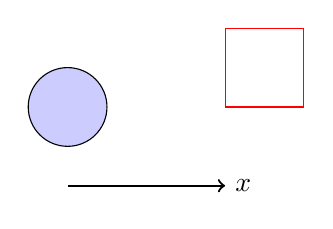
\begin{tikzpicture}
    \draw[thick, ->] (0,0) -- (2,0) node[right] {$x$};
    \draw[fill=blue!20] (0,1) circle (0.5);
    \draw[red] (2,1) rectangle (3,2);
\end{tikzpicture}
\end{lstlisting}

\subsubsection{语法详解 (Syntax)}

\begin{itemize}
    \item \code{\textbackslash draw}: 绘制路径。
    \item \code{(x,y)}: 笛卡尔坐标。
    \item \code{--}: 直线连接。
    \item \code{circle (radius)}: 圆。
    \item \code{rectangle (corner)}: 矩形。
\end{itemize}

\subsubsection{效果展示 (Effect)}

\begin{center}
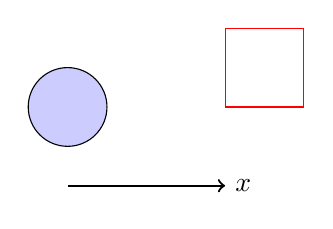
\begin{tikzpicture}
    \draw[thick, ->] (0,0) -- (2,0) node[right] {$x$};
    \draw[fill=blue!20] (0,1) circle (0.5);
    \draw[red] (2,1) rectangle (3,2);
\end{tikzpicture}
\end{center}

\subsection{Flowcharts (流程图)}

\subsubsection{功能介绍 (Introduction)} 

利用 \texttt{otex.sty} 中预定义的样式快速绘制流程图。

Quickly draw flowcharts using predefined styles in \texttt{otex.sty}.

\vspace{0.5em}
\subsubsection{代码展示 (Code)}

\begin{lstlisting}[language=TeX]
\begin{tikzpicture}[node distance=1.5cm]
    \node (start) [startstop] {Start};
    \node (pro1) [process, below of=start] {Process};
    \node (dec1) [decision, below of=pro1] {Check?};
    \draw [arrow] (start) -- (pro1);
    \draw [arrow] (pro1) -- (dec1);
\end{tikzpicture}
\end{lstlisting}

\subsubsection{语法详解 (Syntax)}

\begin{itemize}
    \item \code{\textbackslash node (name) [style] \{text\}}: 定义节点。
    \item \code{below of=node}: 相对定位 (需 \texttt{positioning} 库)。
    \item \code{startstop}, \code{process}, \code{decision}: 预定义样式。
\end{itemize}

\subsubsection{效果展示 (Effect)}

\begin{center}
\begin{tikzpicture}[node distance=1.5cm]
    \node (start) [startstop] {Start};
    \node (pro1) [process, below of=start] {Process};
    \node (dec1) [decision, below of=pro1] {Check?};
    \draw [arrow] (start) -- (pro1);
    \draw [arrow] (pro1) -- (dec1);
\end{tikzpicture}
\end{center}

\subsection{Tree Diagrams (树形图)}

\subsubsection{功能介绍 (Introduction)} 

TikZ 的 \texttt{child} 语法使得绘制树形结构变得非常直观。

TikZ's \texttt{child} syntax makes drawing tree structures very intuitive.

\vspace{0.5em}
\subsubsection{代码展示 (Code)}

\begin{lstlisting}[language=TeX]
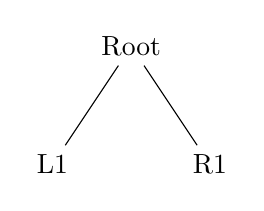
\begin{tikzpicture}[level 1/.style={sibling distance=2cm}]
    \node {Root}
        child { node {L1} }
        child { node {R1} };
\end{tikzpicture}
\end{lstlisting}

\subsubsection{语法详解 (Syntax)}

\begin{itemize}
    \item \code{child \{ node \{...\} \}}: 定义子节点。
    \item \code{sibling distance}: 设置兄弟节点间距。
\end{itemize}

\subsubsection{效果展示 (Effect)}

\begin{center}
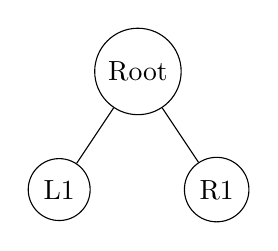
\begin{tikzpicture}[level 1/.style={sibling distance=2cm}, every node/.style={circle,draw}]
    \node {Root}
        child { node {L1} }
        child { node {R1} };
\end{tikzpicture}
\end{center}


\newpage
% ==========================================================
\section{PGFPlots (高级绘图)}
% ==========================================================

\subsection{2D Function Plots (二维函数图)}

\subsubsection{功能介绍 (Introduction)} 

PGFPlots 是基于 TikZ 构建的宏包,专门用于绘制科学数据图表。它提供了坐标轴自动缩放、刻度管理等高级功能。

PGFPlots is a package built on top of TikZ, specifically designed for plotting scientific data. It provides advanced features like automatic axis scaling and tick management.

\vspace{0.5em}
\subsubsection{代码展示 (Code)}

\begin{lstlisting}[language=TeX]
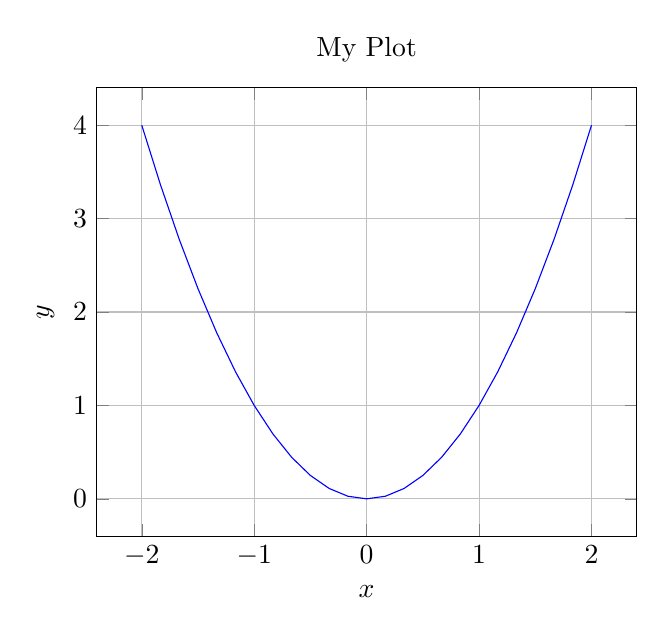
\begin{tikzpicture}
    \begin{axis}[
        title={My Plot},
        xlabel={$x$},
        ylabel={$y$},
        grid=major
    ]
    \addplot[blue, domain=-2:2] {x^2};
    \end{axis}
\end{tikzpicture}
\end{lstlisting}

\subsubsection{语法详解 (Syntax)}

\begin{itemize}
    \item \code{axis}: 坐标轴环境。
    \item \code{\\addplot}: 添加数据系列。
    \item \code{domain}: 定义自变量范围。
\end{itemize}

\subsubsection{效果展示 (Effect)}

\begin{center}
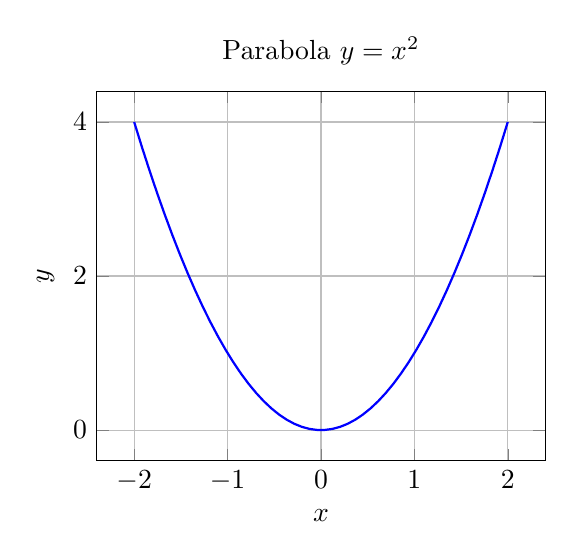
\begin{tikzpicture}
    \begin{axis}[
        width=0.6\textwidth,
        title={Parabola $y=x^2$},
        xlabel={$x$},
        ylabel={$y$},
        grid=major
    ]
    \addplot[blue, thick, domain=-2:2, samples=50] {x^2};
    \end{axis}
\end{tikzpicture}
\end{center}

\subsection{3D Surface Plots (三维曲面图)}

\subsubsection{功能介绍 (Introduction)} 

PGFPlots 还可以绘制令人印象深刻的三维曲面图。

PGFPlots can also draw impressive 3D surface plots.

\vspace{0.5em}
\subsubsection{代码展示 (Code)}

\begin{lstlisting}[language=TeX]
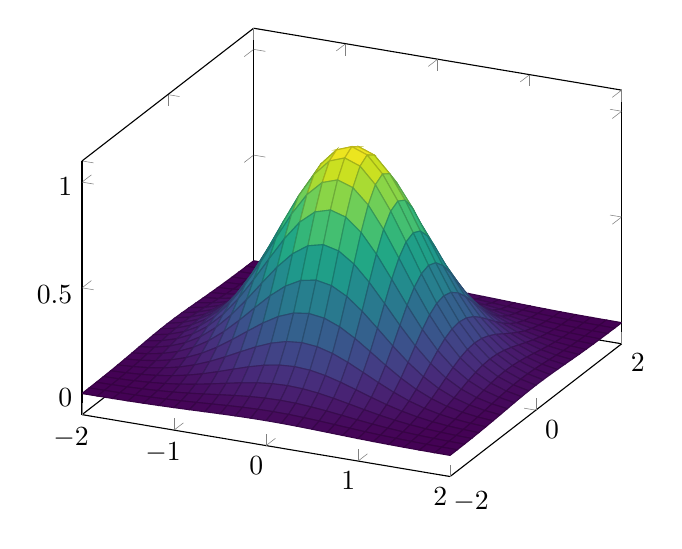
\begin{tikzpicture}
    \begin{axis}[colormap/viridis]
    \addplot3[surf, domain=-2:2] {exp(-x^2-y^2)};
    \end{axis}
\end{tikzpicture}
\end{lstlisting}

\subsubsection{语法详解 (Syntax)}

\begin{itemize}
    \item \code{\\addplot3[surf]}: 绘制三维曲面。
    \item \code{colormap/viridis}: 设置配色方案。
\end{itemize}

\subsubsection{效果展示 (Effect)}

\begin{center}
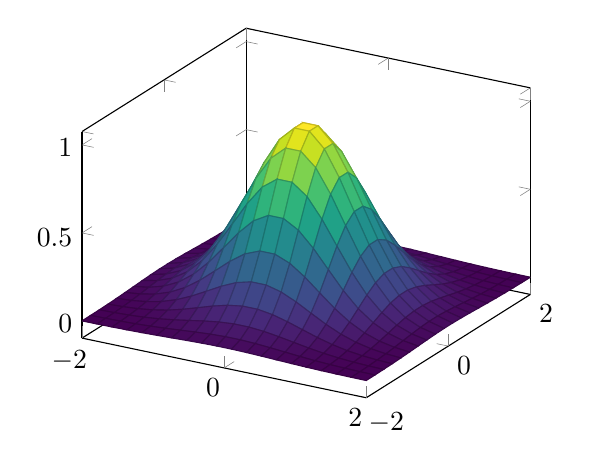
\begin{tikzpicture}
    \begin{axis}[
        width=0.6\textwidth,
        colormap/viridis,
        view={30}{30}
    ]
    \addplot3[surf, domain=-2:2, samples=20] {exp(-x^2-y^2)};
    \end{axis}
\end{tikzpicture}
\end{center}


\newpage
\printbibliography[heading=bibintoc]

\end{document}
